\begin{frame}
	\definecolor{refcol}{RGB}{200, 80, 50}
	\definecolor{matchcol}{RGB}{10, 150, 10}
	\frametitle{\problemtitle}
	\begin{block}{Problem}
		\begin{itemize}
		\item Determine whether pieces of code can be obtained by renaming variables from substrings of a reference
		\vspace{-1.5em}%
		\begin{center}
			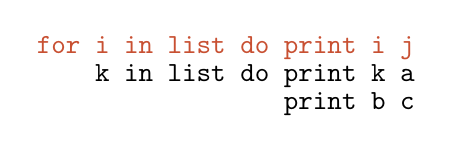
\begin{tikzpicture}
				\node[anchor=west] at (0,0)  (ref) {\textcolor{refcol}{\texttt{\hphantom{}for i in list do print i j}}};
				\node[anchor=west] at (0,-1em) (q) {\texttt{\hphantom{for }k in list do print k a}};
				\node[anchor=west] at (0,-2em) (q) {\texttt{\hphantom{for k in list do }print b c}};
			\end{tikzpicture}
		\end{center}
		\end{itemize}
		\vspace{-0.5em}
	\end{block}
	\pause
	\begin{block}{Solution}
	\begin{itemize}
		\item<+-> Transform the code:

		\vspace{+0.3em}
		\begin{minipage}{0.55\textwidth}
			Replace each occurrence of a variable $V$ with
			\begin{itemize}
				\item<+-> the distance to the previous occurrence of $V$, or
				\item<+-> $0$ if there is no previous occurrence 
			\end{itemize}
		\end{minipage}%
		\begin{minipage}{0.4\textwidth}
			\pause
			\begin{center}
				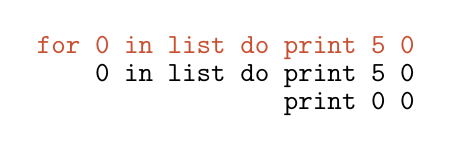
\begin{tikzpicture}	
					\node[anchor=west] at (0,0)  (ref) {\textcolor{refcol}{\texttt{\hphantom{}for 0 in list do print 5 0}}};
					\node[anchor=west] at (0,-1em) (q) {\texttt{\hphantom{for }0 in list do print 5 0}};
					\node[anchor=west] at (0,-2em) (q) {\texttt{\hphantom{for k in list do }print 0 0}};
				\end{tikzpicture}
			\end{center}
		\end{minipage}
		% \item<+-> This (sometimes) deals with the variable renaming
		\item<+-> Do this for all suffixes of the reference:
			\begin{center}
				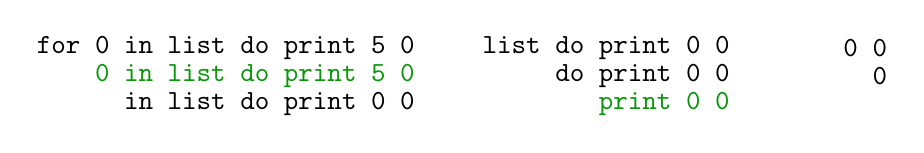
\begin{tikzpicture}	
					\node[anchor=west] at (0,0em)    (r0) {\texttt{\hphantom{}for 0 in list do print 5 0}};
					\node[anchor=west] at (0,-1em)   (r1) {\textcolor{matchcol}{\texttt{\hphantom{for }0 in list do print 5 0}}};
					\node[anchor=west] at (0,-2em)   (r2) {\texttt{\hphantom{for 0} in list do print 0 0}};
					\node[anchor=west] at (4cm,0em)  (r3) {\texttt{\hphantom{for 0 in} list do print 0 0}};
					\node[anchor=west] at (4cm,-1em) (r4) {\texttt{\hphantom{for 0 in list} do print 0 0}};
					\node[anchor=west] at (4cm,-2em) (r5) {\textcolor{matchcol}{\texttt{\hphantom{for 0 in list do} print 0 0}}};
					\node[anchor=west] at (6cm,0em)  (r6) {\texttt{\hphantom{for 0 in list do print} 0 0}};
					\node[anchor=west] at (6cm,-1em) (r7) {\texttt{\hphantom{for 0 in list do print 0} 0}};
				\end{tikzpicture}
			\end{center}
		\item<+-> Sort these transformed suffixes lexicographically, use binary search to find the transformed query
		\item<+-> Time complexity: $\mathcal{O}(n^2 + q \cdot \mathit{qlen} \cdot \log n)$, where $\mathit{qlen} \leq 2\,000$ is the max.\ length of a query
	\end{itemize}
	\end{block}
\end{frame}
